\documentclass[12pt,a4paper]{article}
\usepackage{polski}
\usepackage{graphicx}
\usepackage{secdot}
\usepackage[utf8]{inputenc}
\usepackage[T1]{fontenc}
\usepackage{geometry}
\usepackage{setspace}
\sectiondot{subsection}
\sectiondot{subsubsection}
\makeatletter
\newcommand{\linia}{\rule{\linewidth}{0.4mm}}
\renewcommand{\maketitle}{\begin{titlepage}
    \vspace*{1cm}
    \begin{center}\small
    Sprawozdanie z pracowni problemowej magisterskiej
    \end{center}
    \vspace{3cm}
    \noindent\linia
    \begin{center}
      \LARGE \textsc{\@title}
         \end{center}
     \linia
    \vspace{1cm}
    \begin{flushright}
    \begin{minipage}{5cm}
    \textit{\small Autor:}\\
    \normalsize \textsc{\@author} \\
    \end{minipage}
    \vspace{1cm}
     {\small \\Praca wykonywana pod kierunkiem:}\\
         dra hab. inż. Macieja Ławryńczuka
     \end{flushright}
    \vspace{5cm}
    \begin{center}
    \@date
    \end{center}
  \end{titlepage}%
}
\makeatother
\author{Mateusz Statkiewicz }
\title{Zastosowanie karty graficznej \\(biblioteka CUDA) w optymalizacji\\ z wykorzystaniem \\algorytmów ewolucyjnych
}
\begin{document}
\maketitle
\onehalfspacing
\section{Technologia CUDA}
\linespread{1,3}
\indent CUDA (ang. Compute Unified Device Architecture) jest równoległą architekturą obliczeniową, opracowaną przez firmę NVIDIA. Celem tej technologii jest wykorzystanie mocy układów GPU do rozwiązywania problemów numerycznych efektywniej niż w procesorach ogólnego zastosowania. Architektura jest stosowana w kartach graficznych NVIDII od 2006 roku.
\subsection{Model architektury i pamięci}
\indent W standardowej architekturze karty graficznej przetwarzanie przebiega najpierw przez shader wierzchołków a następnie przez shader pikseli. Każdy z shaderów wykonuje odrębne operacje. W architekturze CUDA jednostki wykonujące obliczenia nie są podzielone na shadery wierzchołków i pikseli, ale są połączone w jeden potok przetwarzania, co pozwala programowi wykonywać obliczenia na wszystkich jednostkach arytmetyczno-logicznych procesora. Jednostki arytmetyczno–logiczne zbudowane są zgodnie z normą IEEE 754, dotyczącą arytmetyki liczb zmiennoprzecinkowych pojedynczej precyzji. Jednostki te posiadają także zestaw instrukcji przeznaczonych do wykonywania ogólnych obliczeń. Dodatkowo, jednostkom wykonawczym GPU zezwolono na swobodny dostęp do pamięci w celu odczytu i zapisu, a także do pamięci wspólnej (zarządzanej programowo pamięci podręcznej). Wszystkie te zmiany w budowie procesorów graficznych zostały wprowadzone, aby procesor GPU nie tylko radził sobie ze standardowymi zadaniami graficznymi, ale i wykonywał ogólne obliczenia. Architektura ma na celu umożliwienie wykorzystania mocy obliczeniowej do rozwiązywania ogólnych problemów numerycznych w sposób wydajniejszy od tradycyjnych, sekwencyjnych procesorów ogólnego zastosowania.
\\\indent CUDA, co najważniejsze, umożliwia przetwarzanie współbieżne - została ku temu specjalnie zaprojektowana. Dlatego też funkcje GPU uruchamiamy w różnych konfiguracjach - to znaczy, że w momencie wywoływania funkcji zobligowani jesteśmy podać liczbę bloków i wątków, na których dany fragment kodu zostanie uruchomiony. Przetwarzanie na karcie graficznej podzielone jest na bloki i zawarte w nich wątki. Wątki w obrębie jednego bloku możemy synchronizować. 
\\\\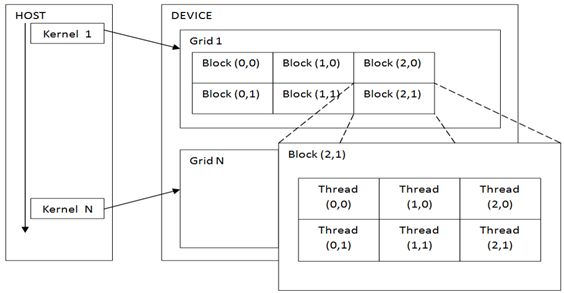
\includegraphics[width=15cm,height=8cm]{img/cuda_arch.jpg}\\
\indent Pamięć karty graficznej została podzielona tak, aby jak najwydajniej z niej korzystać. W funkcjach możemy wykorzystywać ogólną pamięć GPU, np. miejsce, w które kopiujemy dane do przetworzenia. Zakres tej pamięci to wszystkie bloki i wątki uruchamiane na danej karcie graficznej. Kolejnym kontenerem pamięci jest pamięć bloku, czyli pamięć dostępna i współdzielona w obrębie jednego bloku i zawartych w nim wątków. Ostatnim, najmniejszym kontenerem pamięci, jest pamięć wątku, gdzie dostęp ma wyłącznie wątek, dla którego została powołana.
\subsection{Narzędzia pozwalające wykorzystać CUDA}
\indent Integralną częścią architektury CUDA jest oparte na języku C środowisko programistyczne wysokiego poziomu. Składa się ono z: \begin{itemize}
\item nvcc – kompilatora, rozszerzenie gcc;
\item cuda-gdb – debuggera, rozszerzenie gdb;
\item nvprof – profilera;
\item cuda-memcheck – narzędzia do sprawdzania wycieków pamięci,
\item interfejsu programowania aplikacji.
\end{itemize}
Dodatkowym ułatwieniem dla programistów jest dodatek Nsight, dedykowany dla środowisk programistycznych, takich jak Eclipse i Microsoft Visual Studio, umożliwiający korzystanie z wyżej wymienionych narzędzi poprzez interfejs graficzny.
\subsection{CUDA API}
Interfejs programowania aplikacji (ang. API) dla CUDA występuje w 2 formach:
\begin{itemize}
\item NVIDIA CUDA Driver API	 - interfejs niższego poziomu;
\item NVIDIA CUDA Runtime API – interfejs wyższego poziomu.
\end{itemize}
Interfejs niższego poziomu jest trudniejszy do programowania i debugowania, ale oferuje wyższy poziom kontroli i jest niezależny od języka programowania. Trudniej się go konfiguruje i uruchamia. 
W przypadku interfejsu wyższego poziomu, zarządzanie urządzeniem jest ułatwione, gdyż operacje inicjalizacji, zarządzania kontekstem oraz modułami są ukryte i wykonują się automatycznie. Kompilator nvcc generuje kod, wykorzystujący interfejs wyższego poziomu. 
\\\indent Na bazie interfejsu niższego poziomu powstały inne interfejsy. Dzięki temu z możliwości CUDA możemy korzystać za pośrednictwem wielu języków wysokiego poziomu. (Python, Java, .NET, Matlab).
\newpage
\section{Algorytmy ewolucyjne}
\indent Algorytm ewolucyjny opiera się na przetwarzaniu pewnej populacji osobników. Każdy z osobników jest jednym z proponowanych rozwiązań problemu. Algorytm każdemu z osobników przyporządkowuje wartość liczbową opisującą jakość rozwiązania, które dany osobnik reprezentuje. Wartość ta nosi nazwę przystosowania osobnika. Każdy osobnik posiada genotyp - zakodowaną informację jego cech. Genotyp koduje fenotyp który jest bezpośrednio punktem w przestrzeni rozwiązań przeszukiwanego problemu. Przystosowanie jest wynikiem funkcji przystosowania wykonanej na jego fenotypie.\\
\indent Działanie algorytmu sprowadza się do wykonywania 4 kolejnych operacji w pętli. Operacje te to \textit{reprodukcja, operacje genetyczne, ocena} oraz \textit{sukcesja}. Reprodukcja jest operacją wyboru losowych osobników z populacji bazowej. Losowość ta uwzględnia jednak przystosowanie osobników, a co za tym idzie większe prawdopodobieństwo powielenia ma osobnik o lepszym przystosowaniu. Osobniki powstałe w poprzednim etapie poddawane są operacjom genetycznym, które losowo modyfikują ich genotyp. Podstawowe operacje genetyczne to mutacja i krzyżowanie. Mutacja polega na perturbacji genotypu jednego osobnika. Krzyżowanie zaś jest operacją wykonywaną na co najmniej dwóch osobnikach prowadzącą do wygenerowania co najmniej jednego osobnika. Chromosomy nowego osobnika powstają poprzez wymieszanie odpowiednich chromosomów rodzicielskich. Wynikowe osobniki operacji genetycznych nazywamy populacją potomną. Populacja ta jest poddawana ocenie poprzez funkcje przystosowania. Ostatnim etapem jest sukcesja - wybór osobników do nowej populacji bazowej. Do nowej populacji bazowej mogą trafić zarówno osobniki z populacji potomnej jak i bazowej. 
\subsection{Prosty algorytm genetyczny}
\indent J. Holland w 1975 roku zaproponował algorytm modelujący proces ewolucji. Schemat tego algorytmu obecnie nazywamy prostym algorytmem genetycznym. Algorytm ten wykonuje dzialania na dwóch populacjach (bazowej i potomnej) przy pomocy populacji tymczasowej. Schemat oparty jest na 7 krokach:
\begin{enumerate}
\item inicjalizacja populacji bazowej (generacja losowych osobników)
\item ocena populacji bazowej
\item sprawdzenie warunku STOPu, a w razie spełnienia zakończenie algorytmu
\item reprodukcja populacji bazowej do populacji tymczasowej
\item utworzenie populacji potomnej poprzez operacje genetyczne na populacji tymczasowej
\item ocena populacji potomnej
\item przypisanie populacji potomnej jako bazowej dla kolejnej iteracji i powrót do punktu 3.
\end{enumerate}
Warunkiem stopu może być otrzymanie osobnika lepiej przystosowanego niż zadane przystosowanie lub wykonanie określonej liczby iteracji.
\subsection{Strategie ewolucyjne}
\indent Strategie ewolucyjne podobnie jak algorytmy genetyczne operują na populacjach potencjalnych rozwiązań. Korzystają również z zasad selekcji i przetwarzania osobników najlepiej przystosowanych. Między tymi 2 podejściami istnieje jednak wiele różnic.\\ 
\indent Pierwszą z nich jest sposób reprezentacji osobników. W algorytmach genetycznych osobnik reprezentowany jest przez wektor binarny. W strategiach ewolucyjnych wykonujemy działania na osobnikach opartych na wektorze liczb zmiennoprzecinkowych.\\
\indent Kolejna różnica jest ukryta w fazie selekcji. W algorytmach genetycznych do populacji potomnej wybierana jest pewna liczba osobników odpowiadająca liczności populacji bazowej. W strategiach ewolucyjnych tworzona jest populacja tymczasowa, której wielkość może różnić się od wielkości populacji bazowej. Wybór osobników nowej populacji bazowej opiera się wyłącznie na ocenach osobników obliczanych na podstawie funkcji przystosowania. Wybieramy tylko najlepszych osobników (bez powtórzeń). Wybór ten jest deterministyczny. W przypadku algorytmów genetycznych wybór nowej populacji opierał się na losowości, a lepsze osobniki mogły być wybierane kilkukrotnie. \\
\indent Następną różnicą jest kolejność operacji algorytmu. W przypadku strategii ewolucyjnych na początku wykonujemy operacje reprodukcji, a następnie selekcji. Potomek jest rezultatem operacji genetycznych. Utworzona w ten sposób populacja tymczasowa podlega operacji selekcji - zostaje zmniejszona do rozmiaru populacji rodziców. W przypadku algorytmów genetycznych operacje genetyczne wykonywane sa na wyselekcjonowanej populacji tymczasowej.\\
\indent Ostatnią dość istotną różnicą jest samoadaptacja parametrów w strategiach ewolucyjnych, czego nie oferują nam algorytmy genetyczne. Algorytmy te bazują na stałych paramterach operacji genetycznych, podczas gdy w strategiach ewolucyjnych parametry te ulegają ciągłej zmianie. 
\indent Strategie ewolucyjne podzielono na kilka podstawowych typów.
\subsubsection{Strategia (1+1)}
\indent Strategia (1+1) jest algorytmem, na podstawie którego powstały pozostałe strategie. Dlatego jest ona dosyć prosta. W tej strategii przetwarzany jest tylko jeden osobnik. W każdym kroku generowany jest nowy osobnik poprzez mutacje osobnika bazowego. Następnie z tych osobników wybierany jest lepiej przystosowany i to on staje się osobnikiem bazowym kolejnej generacji. Mutacja opiera się na parametrze $\sigma$, który jest odchyleniem standardowym rozkładu normalnego z jakiego losowany jest wektor mutacji.
\indent Do wyboru wartości $\sigma$ zaproponowano algorytm zwany regułą 1/5 sukcesów: \begin{enumerate}
\item jeżeli przez kolejnych k generacji liczba mutacji zakończonych sukcesem (nowy osobnik okazał się lepszy) jest większa od 1/5 ogolnej liczby wykonanych mutacji to należy zwiększyć zasięg mutacji ($\sigma' = c_i\sigma$),
\item jeżeli dokładnie 1/5 ogolnej liczby wykonanych mutacji kończy się sukcesem $\sigma$ nie wymaga korekty,
\item w pozostałych przypadkach zawężamy zasięg mutacji ($\sigma' = c_d\sigma$)
\end{enumerate}
Wartość 1/5 została dobrana na podstawie rozwarzań teoretycznych przeprowadzonych na wielowymiarowych funkcjach testowych. Parametry modyfikujące zostały dobrane eksperymentalnie ($c_d = 0.82, c_i = 1/0.82$)
\subsubsection{Strategia (1+$\lambda$)}
\indent Strategia (1+$\lambda$) jest algorytmem bardzo podobnym do strategii (1+1). Jedyną różnicą jest generacja wielu osobników potomnych. Osobnikiem bazowym nowej generacji jest najlepiej przystosowany ze zbioru wszystkich potomnych i bazowego. Algorytm ten powstał w odpowiedzi na niewielką odporność strategii (1+1) na minima lokalne.
\subsubsection{Strategia ($\mu$+$\lambda$)}
\indent Strategia ($\mu$+$\lambda$) jest jednym z najczęściej wykorzystywanych schematów. Strategia te operuje na populacjach. Populacja bazowa zawiera $\mu$ osobników. Z populacji bazowej generuje sie populację potomna zawierającą $\lambda$ osobników. Proces reprodukcji wygląda następująco: wybiera się populację tymczasową poprzez powtarzanie losowania ze zwracaniem z populacji bazowej. Następnie populacje tymczasową poddaje się operatorom genetycznym (mutacji i krzyżowaniu) otrzymując mutację potomną. Na koniec wybiera się $\mu$ najlepszych osobników z sumy zbiorów populacji bazowej i potomnej (czyli $\mu$+$\lambda$ osobników) tworząc nową populację bazową. \\
\indent Do strategii został wprowadzony mechanizm samoczynnej adaptacji zastępujący regułę 1/5 sukcesów. Na potrzeby tego mechanizmu osobnik został rozszerzony o wektor $/sigma$ - wartości odchyleń standardowych wykorzystywany podczas mutacji. Algorytm przyjmuje dodatkowe 2 parametry ($\tau, \tau'$) wykorzystywane podczas mutacji. Mutacja wykonywana jest w 3 etapach. w pierwszym losowana jest jedna zmienna losowa o jednowymiarowym rozkładzie normalnym ($\xi_{N(0,1)}$), następnie dla każdego elementu wektora $\sigma$ zmienna o tym samym rozkładzie ($\xi_{N(0,1),i}$). Drugi etap to modyfikacja wartości standardowych odchyleń osobnika ($\sigma_i' = \sigma_i$ exp($\tau'\xi_{N(0,1)})+\tau\xi_{N(0,1),i}$ )). Ostatni krok mutacji to zastosowanie nowych odchyleń standardowych na wektor X, czyli wektor zmiennych niezależnych. \\
\indent Krzyżowanie osobników polega na uśrednianiu kolejnych wartości wektora na podstawie rodziców, z parametrem losowanym z rozkładu jednostajnego ( $X' = aX^1+(1-a)X^2$, $\sigma' = a\sigma^1+(1-a)\sigma^2$ , gdzie $a = \xi_{U(0,1)}$). \\
\subsubsection{Strategia ($\mu$, $\lambda$)}
\indent Strategia ta powstała jako wynik spostrzeżenia wady strategii ($\mu$+$\lambda$). Występuje ona kiedy w populacji znajdzie się osobnik o wyróżniającej się wartości przystosowania, ale nieodpowiednich wartościach odchyleń. Taki osobnik nie zostanie usunięty z populacji dopóki nie zostanie znaleziony lepszy od niego. Osobnik ten wpływa niekorzystnie na potomstwo, ponieważ jego nienajlepsze wartości odchyleń są utrwalane i powielane w populacji. Aby zapobiec podobnym problemom zdecydowano się opracować strategię, która pozwoli żyć osobnikowi tylko przez 1 generację. A więc jedyna różnica między tymi strategiami to wybór nowej populacji bazowej odbywa się poprzez selekcję najlepszych $\mu$ osobników spośród $\lambda$ osobników potomnych, a nie z sumy zbiorów populacji potomnej i bazowej jak to odbywało się w strategii ($\mu$+$\lambda$).
\newpage
\section{Postępy pracy}
\indent Celem pracy jest stworzenie aplikacji pozwalającej użytkownikowi przeprowadzanie optymalizacji zdefiniowanych funkcji różnymi metodami ewolucyjnymi. Aplikacja zostanie napisana w językach C/C++/CUDA C z wykorzystaniem standardowych bibliotek systemowych oraz bibliotek pakietu CUDA. Dodatkowym założeniem jest wykorzystanie w implementacji interfejsu aplikacji biblioteki Qt.\\
\indent Dotychczas zapoznałem się z biblioteką CUDA, wraz z CUDA Runtime API. Zaimplementowałem również opisane w tym dokumencie strategie ewolucyjne w wersji dla CPU.\\
\indent W najbliższym czasie planuje "przepisać" implementacje strategii na kod wykonywany przez kartę graficzną, oraz dostosować je do uruchamiania z aplikacji. Zapoznać się z biblioteką Qt w stopniu wystarczającym do stworzenia aplikacji. 
\begin{thebibliography}{9}

\bibitem{arabas05}
	Arabas J.,
	\emph{Wykłady z algorytmów ewolucyjnych}.
	Wydawnictwa Naukowo-Techniczne, 
	Warszawa,
	2004.

\bibitem{sanders10}
	Sanders J., Kandrot E., 
	\emph{CUDA by example. An Introduction to general-purpose GPU Programming}.
	Pearson Education, Michigan, 
	2010.

\bibitem{rutkowski05}
	Rutkowski L.,
	\emph{Metody i techniki sztucznej inteligencji}.
	Wydawnictwo Naukowe PWN, 
	Warszawa,
	2005.

\bibitem{cudaDoc}
	Dokumentacja bibliotek i narzędzi CUDA Toolkit 
	(\emph{http://docs.nvidia.com/cuda/index.html}) – konsultacja dn. 15.05.2014.

\end{thebibliography}
\end{document}
